\chapter*{The Graphical User Interface}
\label{cha:gui}

This chapter describes the RFSM IDE\footnote{Screenshots used in this chapter show the Windows
  version of the RFSM IDE. The IDE can also be built and used on Unix-based systems (Linux,
  MacOS).}. This IDE basically provides a Graphical user Interface (GUI) to the \verb|rfsmc|
compiler described in chapter~\ref{cha:rfsmc}.

\medskip
The GUI allows
\begin{itemize}
\item writing, reading and editing of RFSM programs,
\item generating and viewing graphical representations of these programs,
\item running simulations,
\item generating C, SystemC and VHDL code.
\end{itemize}

\medskip
\textbf{Note}. This chapter supposes that the IDE has been correctly installed. If not, refer to the
installation guide provided in the RFSM distribution.

% \bigskip
% We will illustrate how to write, compile and simulate with the RFSM IDE with the program introduced
% in Listing~\ref{lst:rfsm-example} in chapter~\ref{cha:overview}.

\medskip
First, \textbf{launch the RFSM application} by clicking on its icon in the installation directory or
directly from the Windows \emph{Start} menu. 

% When launched for the first time, the application will display the dialog shown in
% Fig.~\ref{fig:first-launch}. This dialog is used to define the path to the two external programs
% called by the \caphy application :
% \begin{itemize}
% \item the \caph compiler itself,
% \item the program used to visualize the \texttt{.dot} files.
% \end{itemize}
% Enter the complete path to the program in the corresponding text box or use the
% \verb|...| button located at the right of the box to set it.
% If you don't have the \texttt{Graphviz}\footnote{\url{http://graphviz.org}.} installed on your
% machine, leave the second text box blank. Note that you won't be able to visualize the dataflow
% graphs generated by the \caph compiler, however.

% \begin{figure}[h]
%   \centering
%   \includegraphics[width=0.75\textwidth]{figs/ide/ini-dialog}
%   \caption{The dialog shown by \caphy at first launch}
%   \label{fig:first-launch}
% \end{figure}

\medskip
The application main window is shown in Fig.~\ref{fig:main-window}. 
The main elements are (with corresponding areas labeled in red in Fig.~\ref{fig:main-window}) :
\begin{enumerate}
\item a menubar
\item four buttons for file manipulation; from left to right
  \begin{itemize}
  \item create a new file,
  \item open an existing file,
  \item save a file,
  \item save all files.
  \end{itemize}
\item five buttons to invoke the compiler for (from left to right)
  \begin{itemize}
  \item generating graphical representations of the current program and visualize it,
  \item simulating the current program and visualize it,
  \item generating C code from the current program,
  \item generating SystemC code from the current program,
  \item generating VHDL code from the current program (button \textsc{VHDL}).
  \end{itemize}
\item a tab for viewing and editing input source files,
\item a tab for viewing output files,
\item a log area, displaying issued command and outputs from the compiler.
\end{enumerate}

\begin{figure}[h]
  \centering
  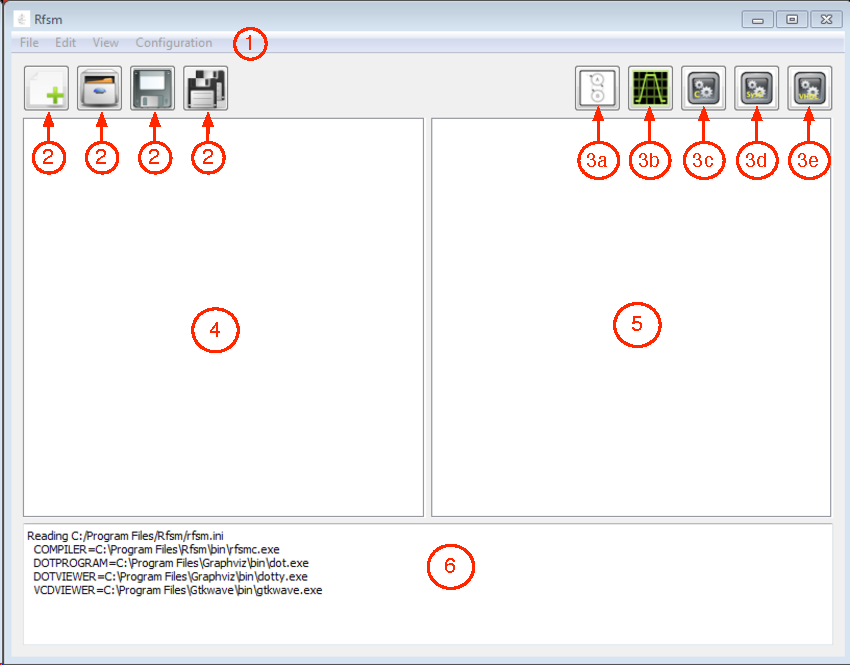
\includegraphics[width=0.75\textwidth]{figs/gui/mainwindow}
  \caption{Main window of the RFSM application}
  \label{fig:main-window}
\end{figure}

\medskip
Invoke the [\textsf{Configuration:Compiler and Tools}] menu item and check that the specified paths
are right (see Fig.~\ref{fig:config-window}). They should respectively point to 
\begin{itemize}
\item the location of the \texttt{rfsmc} compiler (\verb|<install>/bin/rfsmc|, where
  \verb|<install>| is the RFSM installation directory, as specified during the installation
  process),
\item the location of the program to invoke for processing \verb|.dot| files, 
\item the location of the program to invoke for viewing \verb|.dot| files, 
\item the location of the program to invoke for viewing \verb|.vcd| traces. 
\end{itemize}
If the specified paths are not correct\footnote{This may be the case, for example, if you have
  changed the program to view graphs and/or images since RFSM was installed.}, adjust them and click \textsc{Ok}.

\begin{figure}[h]
  \centering
  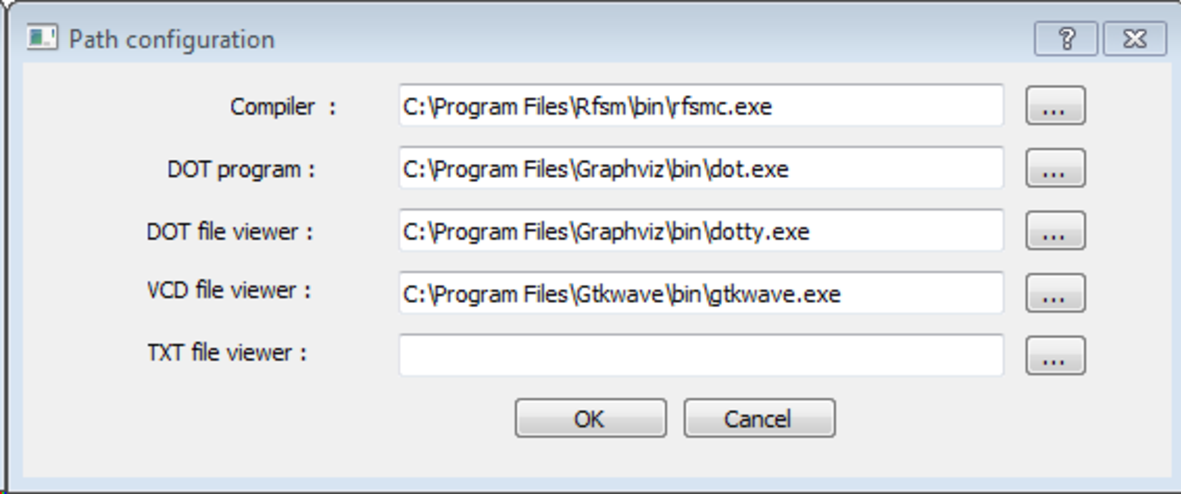
\includegraphics[width=0.75\textwidth]{figs/gui/pathconfig}
  \caption{Path configuration window}
  \label{fig:config-window}
\end{figure}

\medskip \textbf{Create a new source file} or \textbf{open an existing file} by clicking on the
\textsf{New file} (resp. \textsf{Open File}) button 
or invoking the corresponding item of the \textsf{File} menu. A new tab will appear, either blank or
containing the text of the opened file. This file can be freely edited and
saved. Fig.~\ref{fig:first-program} shows the GUI after opening the file containing the example
introduced in Listing~\ref{lst:rfsm-example} of chapter~\ref{cha:overview} (this file is located in directory
  \texttt{examples/single/mousectlr} of the distribution).

\begin{figure}[h]
  \centering
  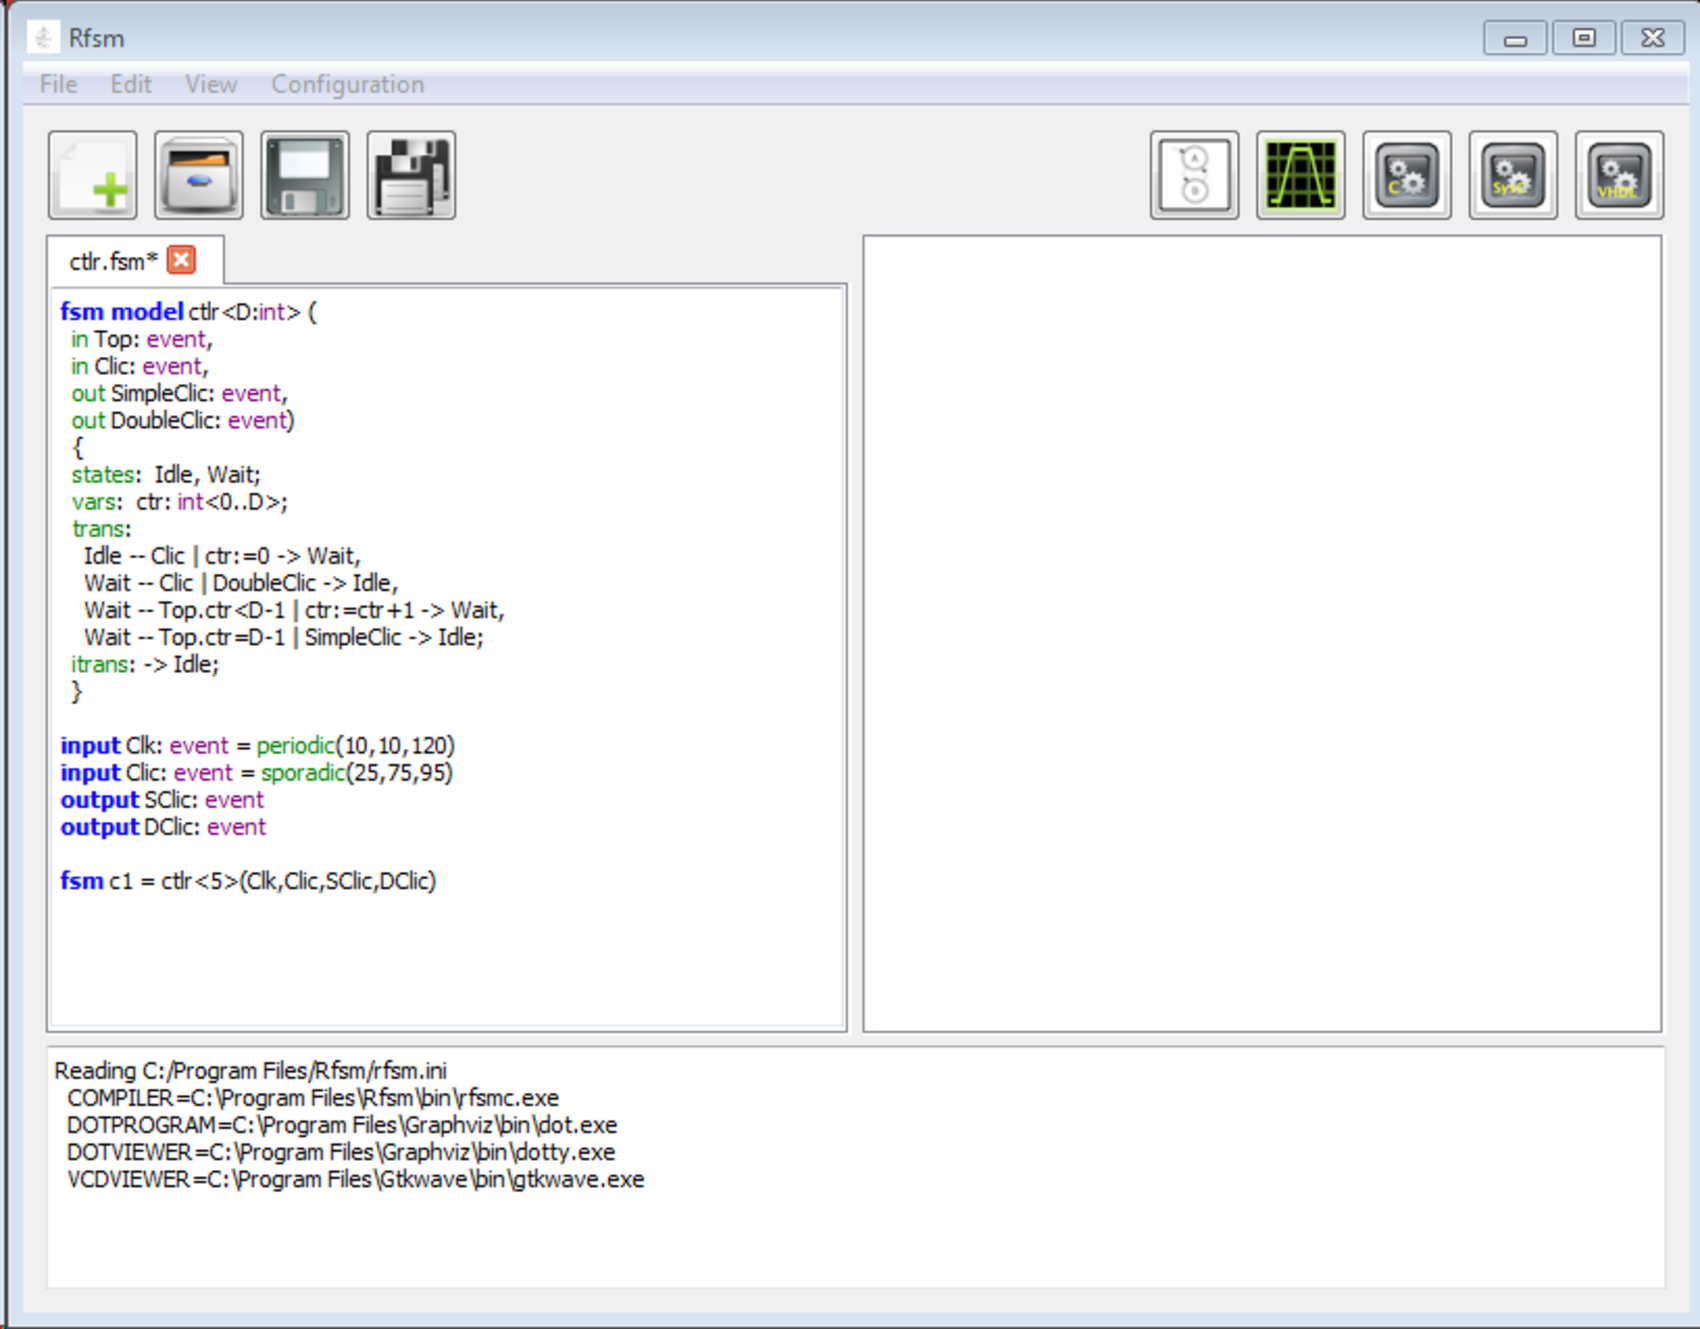
\includegraphics[width=0.75\textwidth]{figs/gui/source}
  \caption{Editing source program}
  \label{fig:first-program}
\end{figure}

\medskip
To \textbf{generate the graphical representation of the program}, click on the \textsf{Graph} button
(numbered \textsf{3a} in Fig.~\pageref{fig:main-window}). This will
\begin{itemize}
\item invoke the \verb|rfsmc| compiler with the adequate option(s),
\item generate the \texttt{.dot} result file (in the same directory as the source file),
\item view this result by invoking the graph visualisation program specified in 
  [\textsf{Configuration : Compiler and Tools}] window.
\end{itemize}

The result is displayed in Fig.~\ref{fig:make-dot}.

\begin{figure}[h]
  \centering
  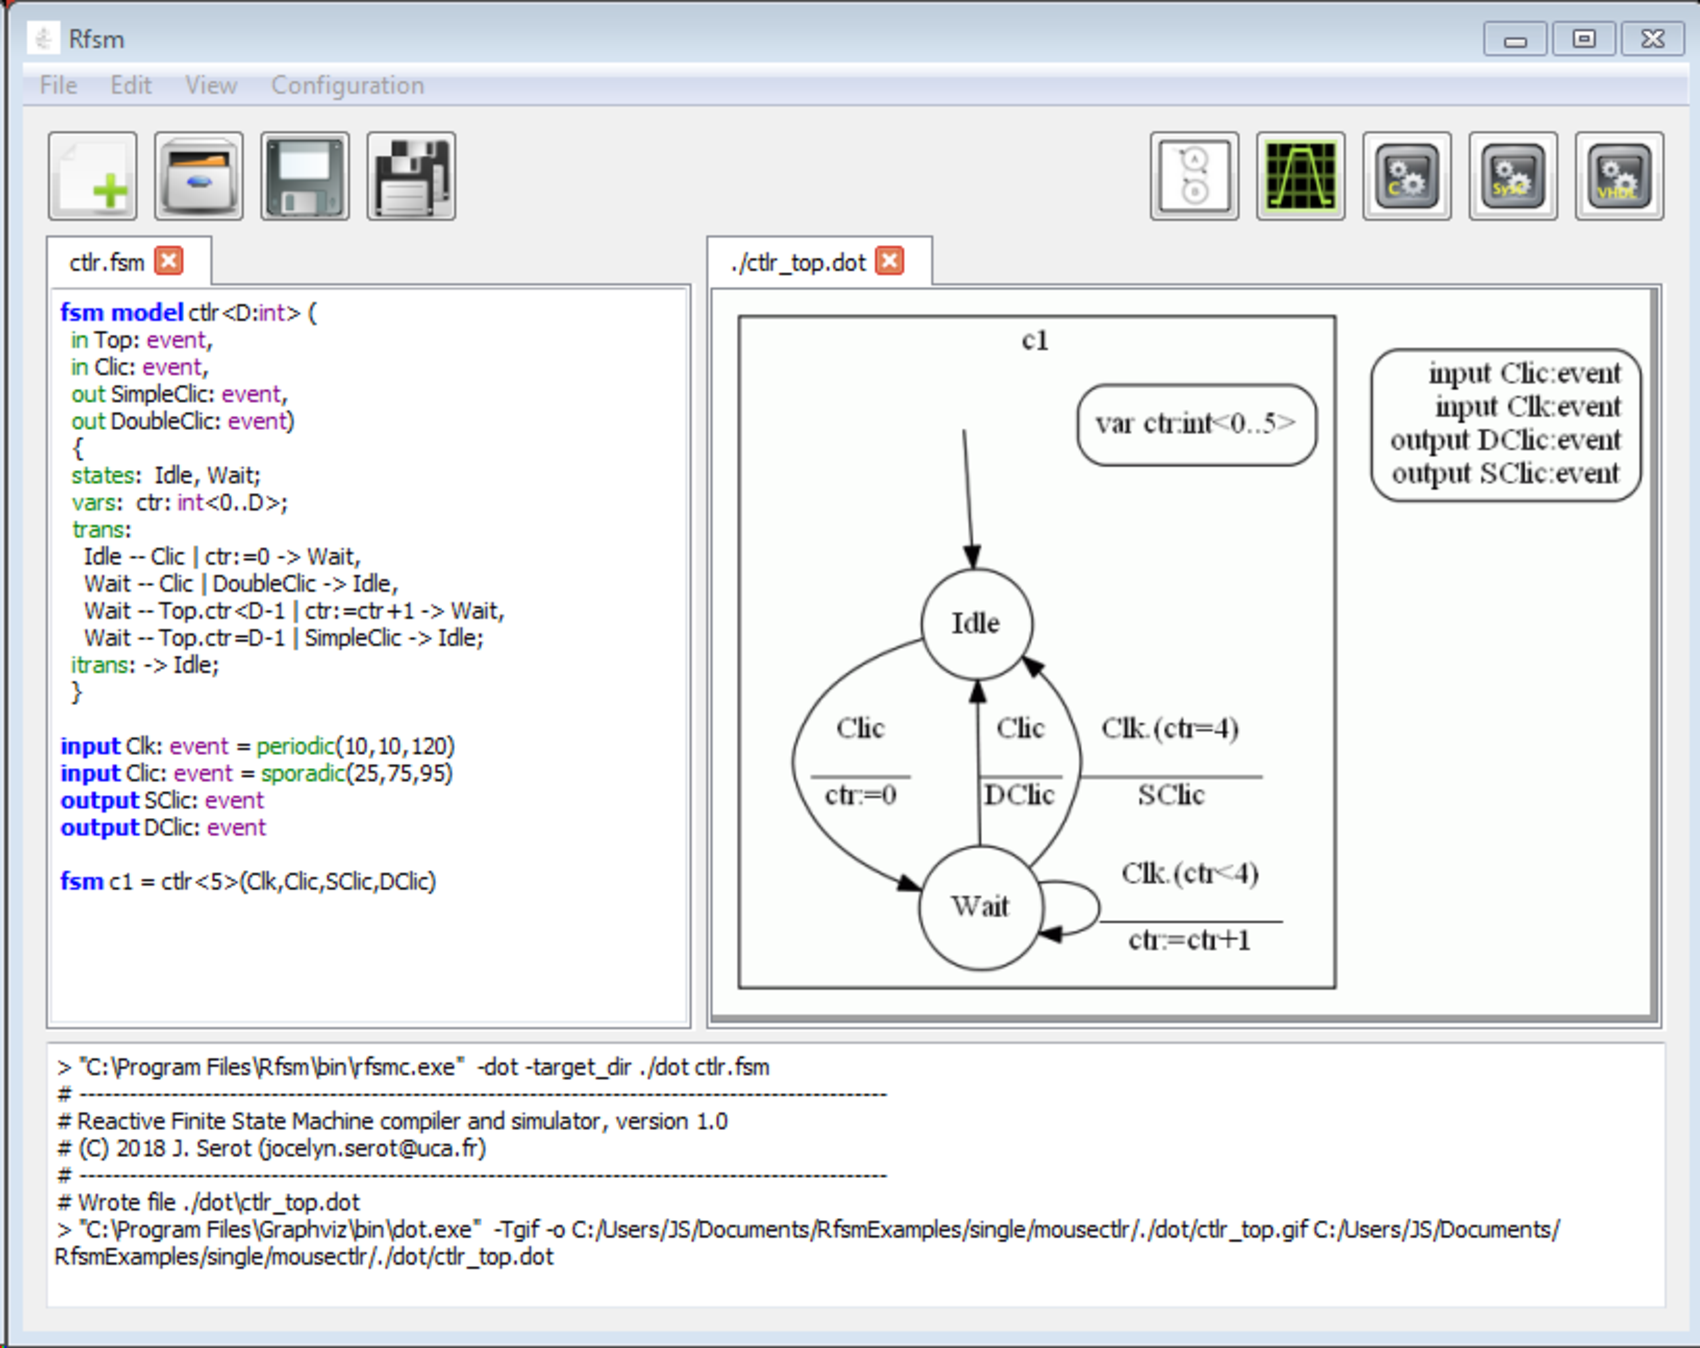
\includegraphics[width=0.75\textwidth]{figs/gui/make-dot}
  \caption{Viewing the graphical representation of the program}
  \label{fig:make-dot}
\end{figure}

\medskip For \textbf{simulating the program}, invoke the compiler by clicking on the \textsc{Sim}
button (numbered 2 in Fig.~\pageref{fig:main-window}). This will run the program, generate results
in the file \texttt{run.vcd} and launch the VCD viewer specified in 
  [\textsf{Configuration : Compiler and Tools}] window.
The result is displayed in Fig.~\ref{fig:make-sim}.

\begin{figure}[h]
  \centering
  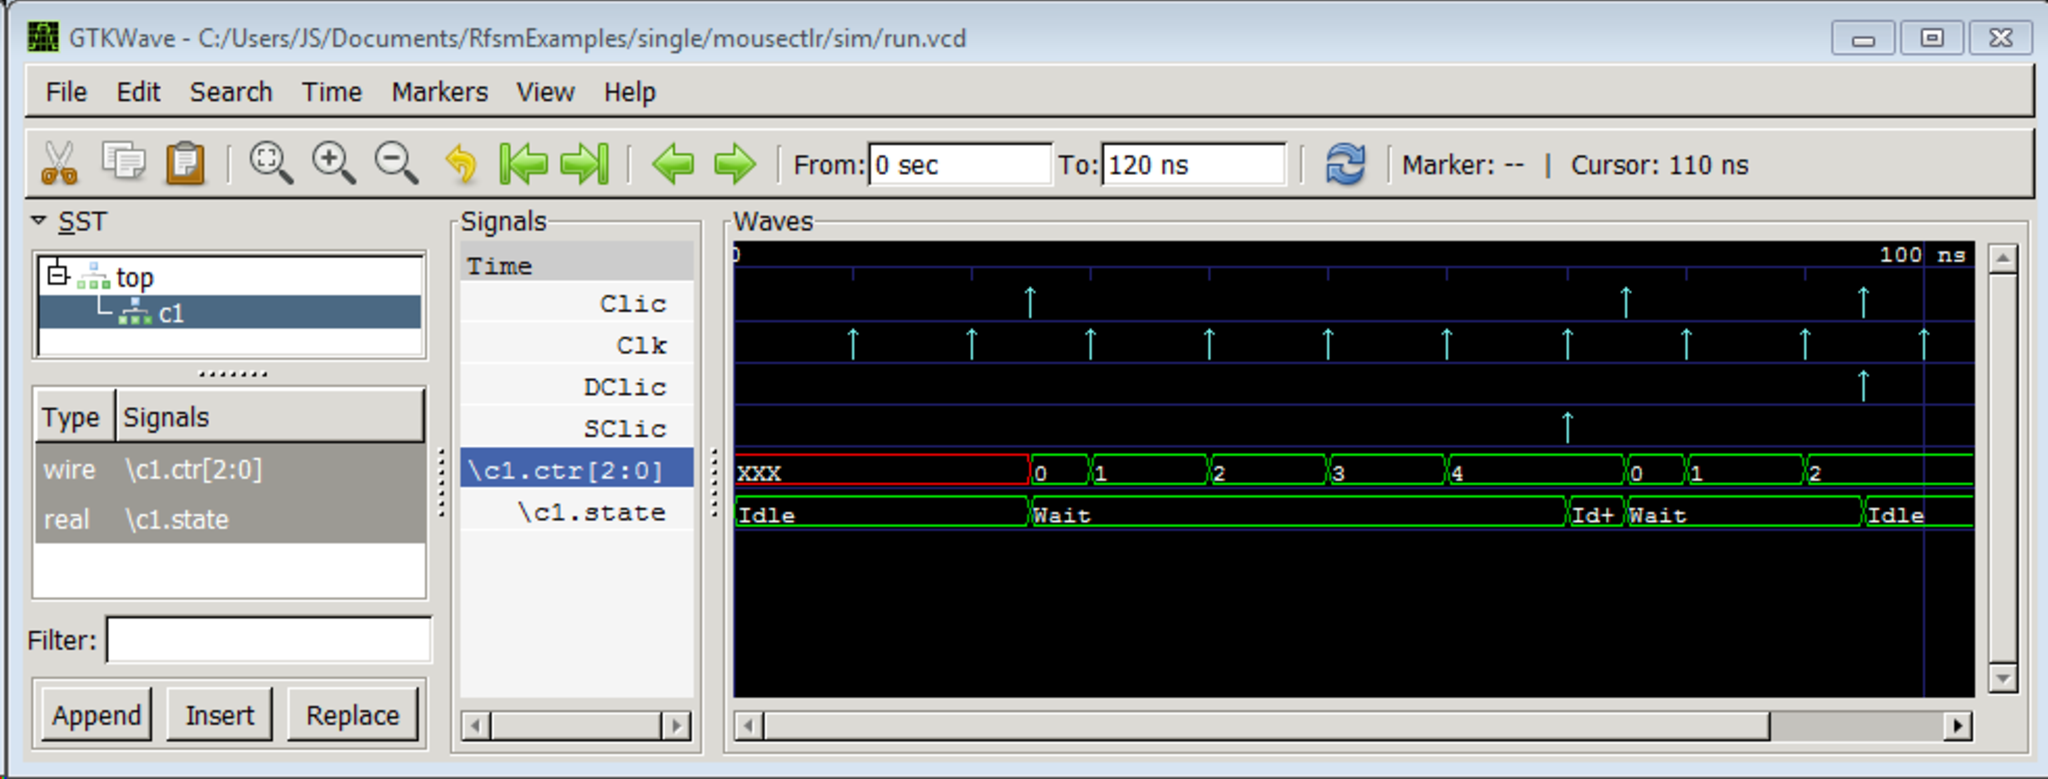
\includegraphics[width=0.75\textwidth]{figs/gui/make-sim}
  \caption{Viewing the simulation result}
  \label{fig:make-sim}
\end{figure}

\medskip
For \textbf{generating the C, SystemC or VHDL} code,
click on the corresponding buttons (numbered \textsf{3c}, \textsf{3d} and \textsf{3e} in
Fig.~\ref{fig:main-window}). The result files will be generated in sub-directories named \verb|./ctask|, \verb|./systemc| and
\verb|./vhdl| and displayed as separate tabs on the
right, as illustrated in Fig.~\ref{fig:make-systemc}, for example.

\begin{figure}[h]
  \centering
  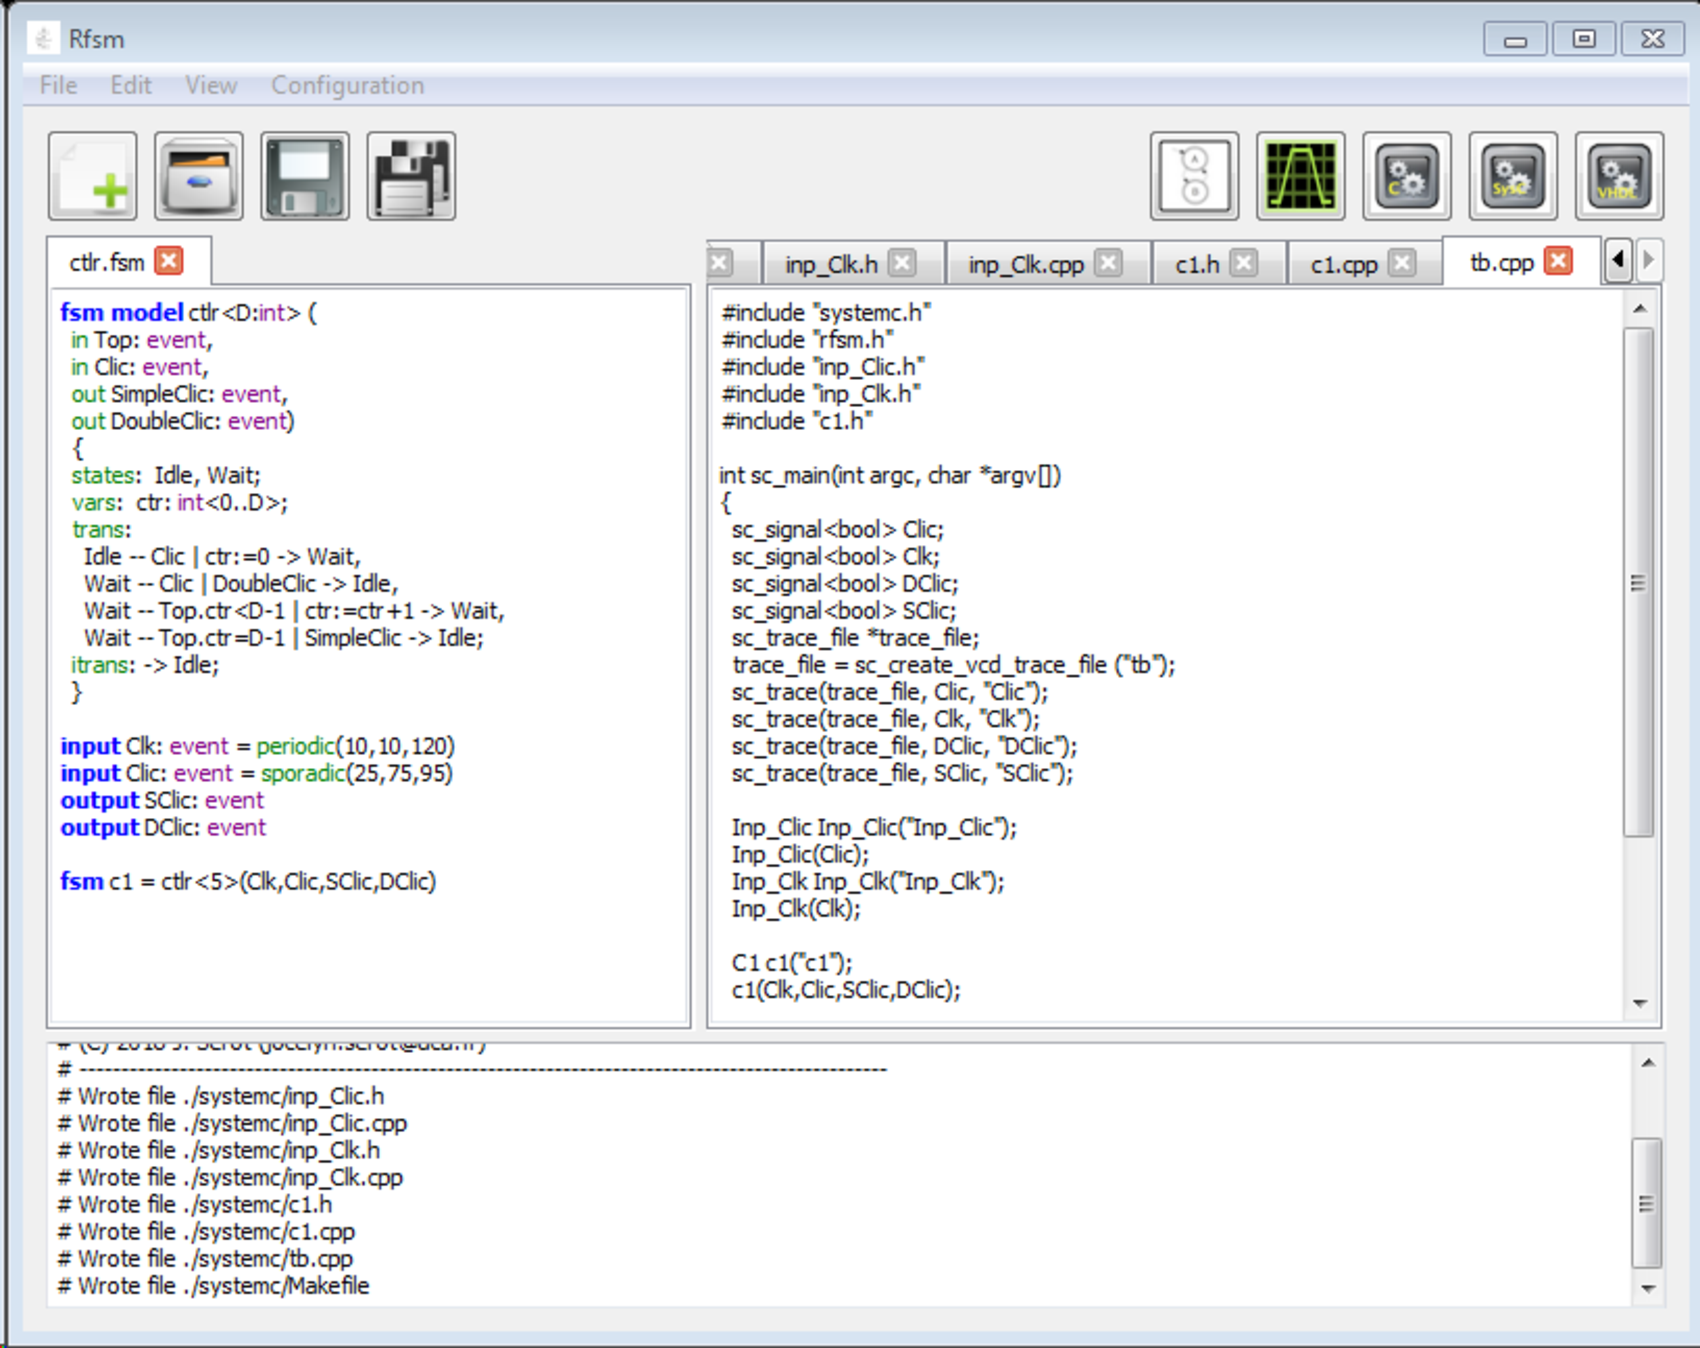
\includegraphics[width=0.75\textwidth]{figs/gui/make-systemc}
  \caption{After generating SystemC code}
  \label{fig:make-systemc}
\end{figure}

\medskip
Options to be passed to RFSM compiler can be set and inspected by invoking \textsf{Compilater options} item of the
\textsf{Configuration} menu, as illustrated in Fig.~\ref{fig:options}. These options are
documented in Appendix B.

\begin{figure}[h]
  \centering
  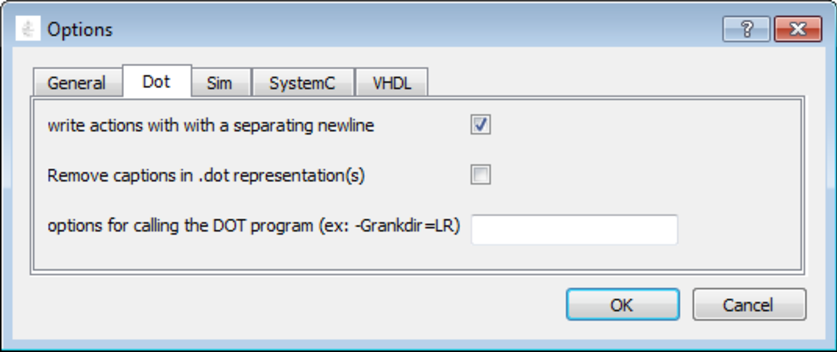
\includegraphics[width=0.75\textwidth]{figs/gui/options}
  \caption{The options setting dialog}
  \label{fig:options}
\end{figure}

%%% Local Variables:
%%% mode: latex
%%% TeX-master: "rfsm"
%%% End:
